\section{Introduction}

\subsection{Problem Definition}

\indent

3D printing technologies offer the ability to produce new parts quickly, allowing faster and cheaper design iterations. However, commercially available Fused Deposition Modeling (FDM) 3D printers currently produce relatively weak parts due to the materials and print method used. They print using weak thermoplastics, most commonly polylactic acid (PLA) or acrylonitrile butadiene styrene (ABS), and deposit the material only in planar layers parallel to the build platform. Because of poor layer adhesion, this method yields parts that fail quickly under loading due to layers being sheared or pulled apart (delamination); this type of failure is particularly evident in parts with thin bosses or shells normal to the build plane, which offer very little surface area for layers to bond. Some parts may be rotated in the printer software to maximize layer contact area, but the planar layer limitation remains. These faults in FDM printers limit much of 3D printing to rapid prototyping applications (where strength is not necessary) despite high demand for printers that can produce stronger parts for use in load-bearing applications. Subsequently, there exists a need for 3D printers using alternative materials and layer formulations that are capable of printing stronger, more usable parts.\\

\subsection{Background Research}

\indent

Current research indicates curved layers as a promising alternative layer geometry and fiber reinforced polymers as stronger  materials for FDM printers. While many resources were used to develop the concept of this 3D printer, a few key sources demonstrated the feasibility and value of the idea.\\

Research into curved layer ABS FDM prints indicates that this layer configuration provides stronger adhesion and better conforms to contoured features. Close to 150\% strength increases were found in parts where critical stresses were located on contoured features. Furthermore, this research demonstrated the problems of using low resolution actuation systems in curved layer FDM, citing difficulty in precisely depositing the material when high-precision, industrial-grade nozzle translation systems are not used \cite{cute-curves}.\\

Research into the strength of carbon fiber cross-ply composites demonstrated dependence of part strength on the fiber angle (between a 0\degree - 90\degree pair and a 45\degree - 45\degree pair) between alternating flat layers. This research, out of the Oak Ridge National Laboratory, showed that tensile strength, shear strength, stiffness, and fatigue varied greatly depending on the cross-ply angles.\footnote{Note that cross-ply composites use long carbon fibers}\cite{ornl} Additional research has analyzed the effects of cross-ply angles \cite{cantilever} in flat FDM ABS parts. Once again, orientation angle played a significant role in the strength of the part. Surprisingly, experimental and theoretical results showed modal solutions (multiple fiber orientations yielding nearly identical peaks in mechanical properties).\\

Finally, one company, MarkForged\cite{markforged}, has come close to realizing the full capability of FDM with a proprietary continuous carbon fiber filament. This company has produced parts that are as strong but slightly less stiff than aluminum. Acquiring a MarkForged printer to help progress this project was initially a goal, but even now they have just started to ship (with multiple-month delays) and are an unreasonably expensive purchase for a senior design project\footnote{\url{https://markforged.com/order-mark-one}}.\\

These crucial sources demonstrate the dependency of part strength on layer type and fiber orientation. They further show the promise of CFRPs, which indicates huge potential for combining CFRP filaments with a curved layer FDM method. With these two methods combined, strong parts made out of carbon fiber could be brought into the homes of general consumers, and industry could begin using 3D printed parts in load-bearing applications rather than for rapid prototyping.\\

\subsection{Project Approach}

\indent

To create stronger 3D printed parts we developed a Curved Layer Carbon Fiber 3D printer. The printer is setup to utilize an FDM technique to deposit one continous strand of custom-developed carbon fiber reinforced plastic (CFRP) filament in curved layers. Using curved layers orients the fiber in the optimal direction(s) for withstanding the applied loads and provides more area for adhesion comprared to a model built with planar layers. To achieve curved layers a serieal robot arm with six degrees of freedom is used instead of a typical cartesian coordinate robot. These extra degrees of freedom allow the robot to lay the CFRP filament in the orientation(s) required for optimized mechanical properties. Finally, once parts are printed, experimental tests can quantify the strength and stiffness increases of curved layer CFRP parts compared to tradiational planar ABS components.\\

With only on academic year to develop this curved layer carbon fiber, efforts were placed on fully setting up the 3D printing tool chain, acquiring and programming a 6-DOF manipulator, and printing one specific part (shown with applied loads in Figure~\ref{fig:intro-layers-geometry-loads}. The bridge geometry was selected due to its reoccurance in academic papers exploring curved layer FDM methods \cite{cute-curves}. Additionally, the strength of this specimen can easily be tested at Cooper by mounting the two flat ends in the Instron (a machine for axial load testing) jaws (Figure~\ref{fig:instron-close-up}) and performing a compression test to induce bending in the arch to quantify the part's mechanical properties.\footnote{In parts with planar build layers, limited adhesion area causes premature failure. However, in curved layer CFRP parts the fibers carry most of the load and adhesion area is maximized.}\\

\begin{figure}[h!]
\centering
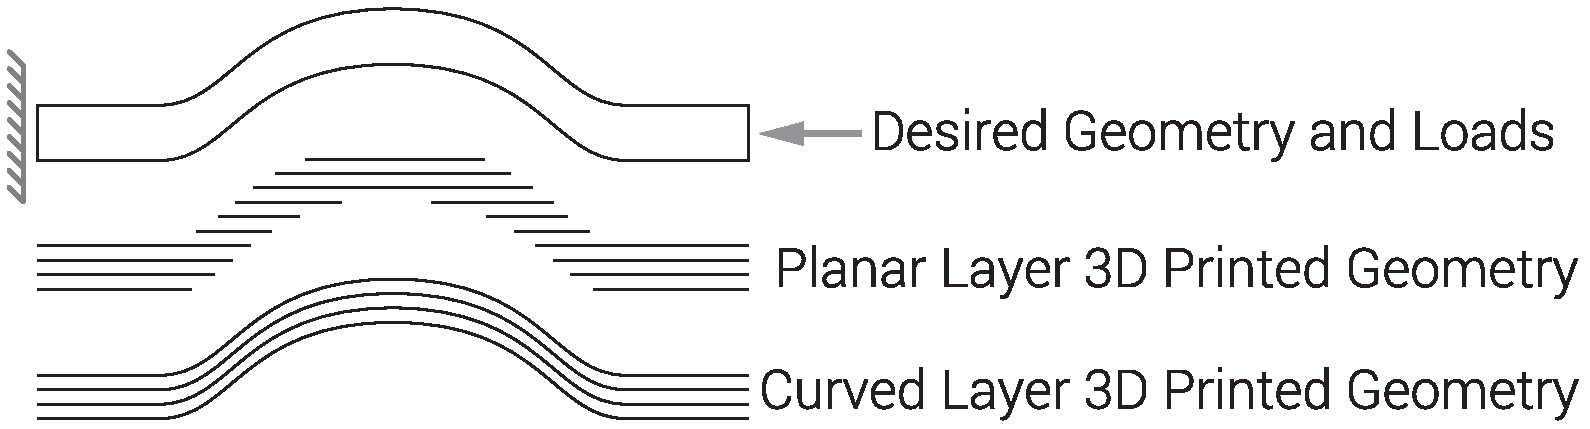
\includegraphics[width=0.7\textwidth]{./figures/intro-layers-geometry-loads}
\caption{3D printing layer discretization methods. The desired part (top), typical planar/cartesian layers (middle), and curved layers (bottom).}
\label{fig:intro-layers-geometry-loads}
\end{figure}

\begin{figure}[h!]
\centering
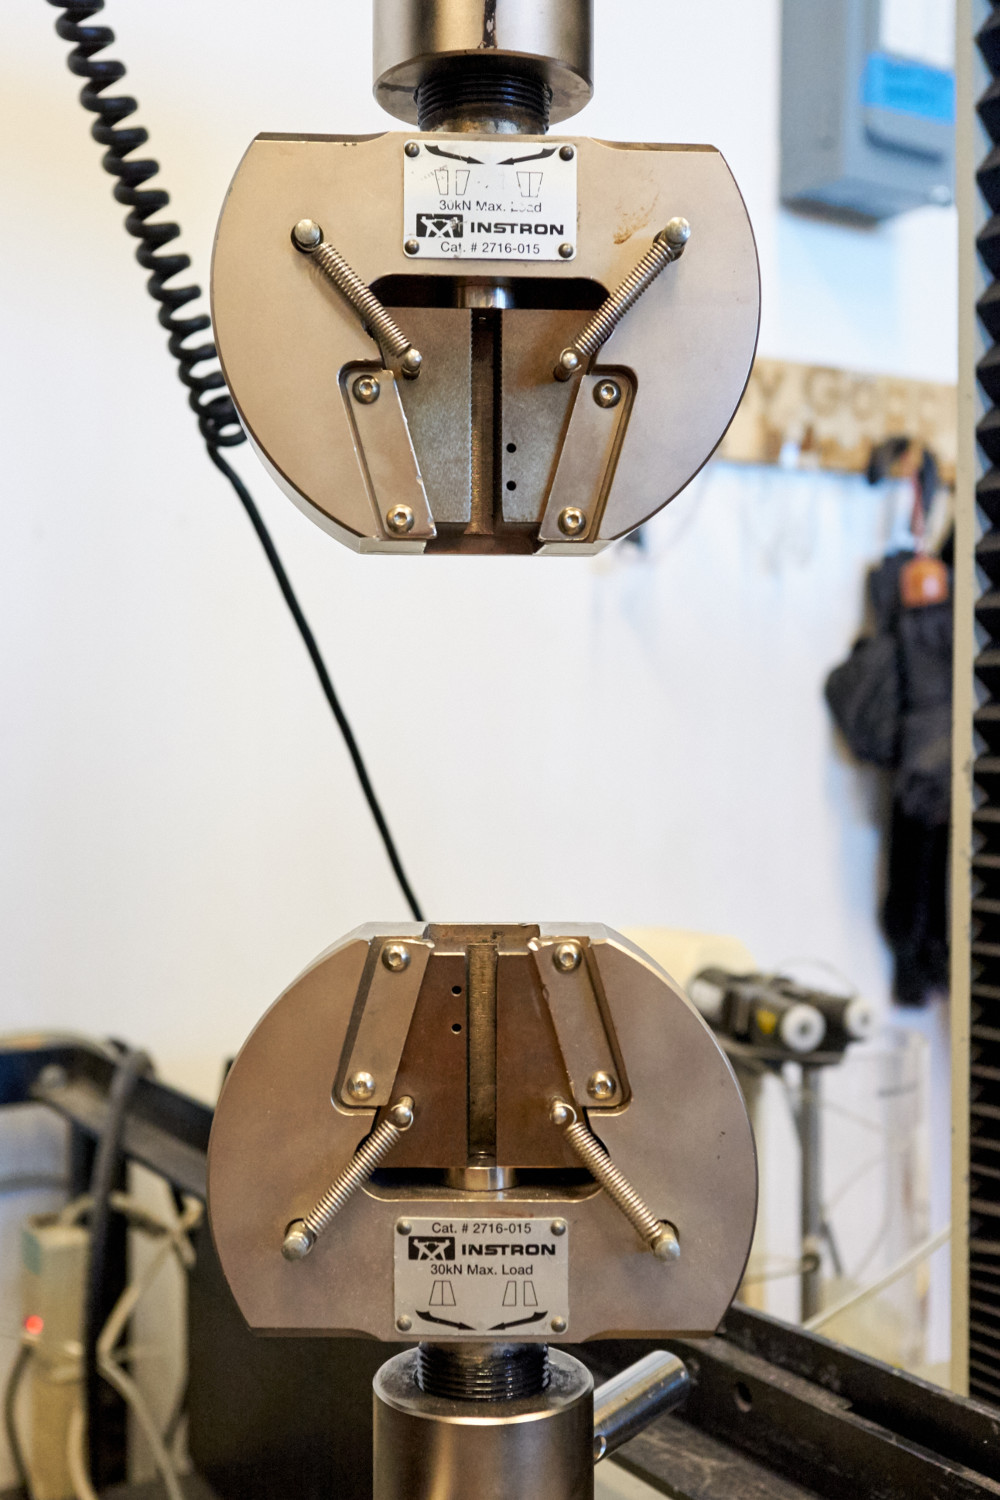
\includegraphics[width=0.5\textwidth]{./figures/instron-close-up}
\caption{A close up view of the Intron jaws used for clamping parts in tension and compression tests.}
\label{fig:instron-close-up}
\end{figure}

To accomplish these goals, a FANUC LR Mate 200iC industrial robot was aquired and programmed with geometry-specific toolpaths. Additional hardware was installed into the robot system to power and control the extruder, and to access tool centerpoint speed data from the robot. With these additions, volumetric flow rate of the filament is matched to the speed to keep the extrusion rate per unit length constant. An extruder end-effector was designed and fabricated to mount to the FANUC's robotic grip and accomodate a CFRP filament. A novel CFRP filament was experimentally developed and test printed. Finally, a finite element analysis of the bridge specimen was performed to predict the strength of the speciment and determine optimal fiber orientation. Figure~\ref{fig:poster-image} shows a photograph of 3D printer. With the framework for the printer completely liad out, it is our hope that the curved layer carbon fiber printer is picked up as a senior project next year where students print and mechanically test the sample and other specimen, implement minor adjustments to the setup to achieve maximum part strength based on experimental findings, and ultimately print the next generation of 3D printed parts.\\

\begin{figure}[h!]
\centering
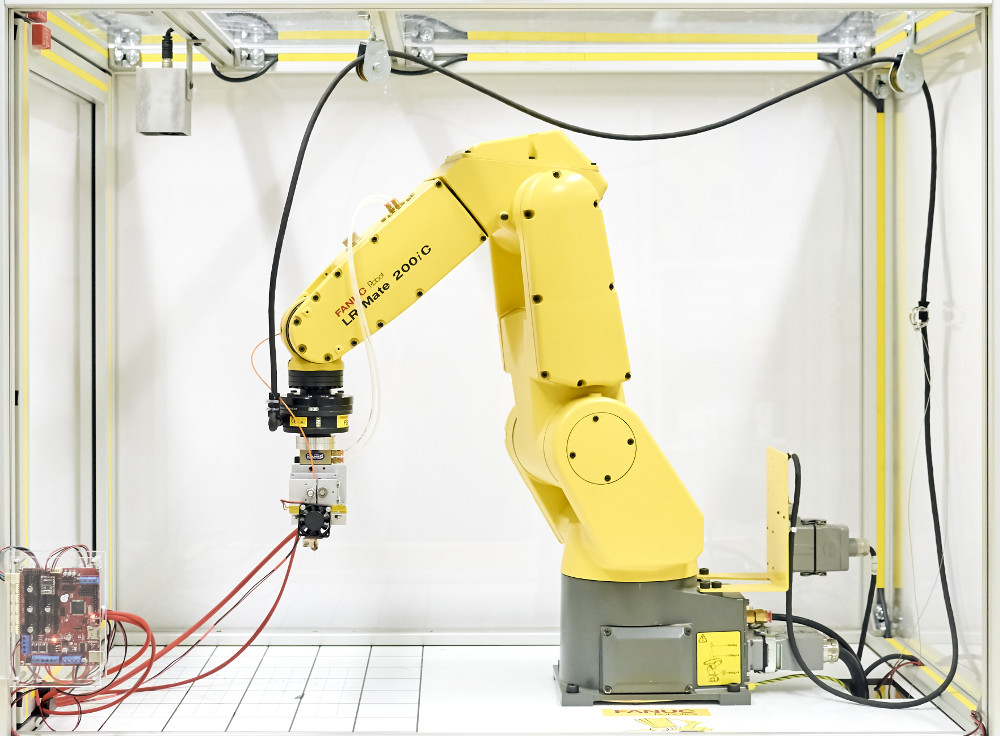
\includegraphics[width=0.8\textwidth]{./figures/poster-image}
\caption{An overview image of the curved layer carbon fiber 3D printer.}
\label{fig:poster-image}
\end{figure}

%To create stronger 3D printed parts we are developing a Curved Layer Carbon Fiber 3D Printer. The printer will utilize FDM techniques to deposit one continuous strand of a carbon fiber reinforced plastic (CFRP) filament in curved layers. This material will mirror existing, widely used fiber-reinforced polymer materials, such as carbon fiber and fiberglass composites. Using curved layers will orient fibers in optimal direction(s) for withstanding applied loads and provide more area for layer adhesion. Figure~\ref{fig:layers} shows how curved layers compare to the typical cartesian layer method. To achieve curved layers a serial robot arm with six degrees of freedom will be used instead of a typical cartesian coordinate robot. These extra degrees of freedom will allow the printer to lay material in any direction. In combination with precise control over toolpaths, the CFRP filament and curved layers will allow strong fibers to be oriented optimally for the desired mechanical properties of the part. These properties will be user-determined based on expected loading, surface finish, and other part requirements. Ultimately, experimental comparisons between curved layer FDM and standard FDM parts will quantify the increase in strength and provide additional insights towards optimizing fiber orientation.\\

%To realize the goal of a fiber-reinforced composite curved layer 3D printer, the project was broken down into five subsystems, which are outlined in Figure~\ref{fig:flowchart}. First, all components of the 3D printing toolchain must be developed. The toolchain is defined by any hardware or software necessary for the steps between receiving a STereoLithography file (STL) and the printed part, which includes but is not limited to the extruder, control electronics, and the tool path generation scheme. Second, we must locate and learn to control a robot arm capable with six degrees of freedom. Third an appropriate CFRP with a usable ratio carbon fiber and thermoplastic matrix material is to be created. Fourth, computational and experimental methods can be utilized to determine optimal fiber orientation based on user requirements. Fifth, the printed parts will be experimental tests to quantify their mechanical properties. These five subsystems will come together to fully create the curved layer carbon fiber 3D printer.
%
%\begin{figure}[htp]
%\centering
%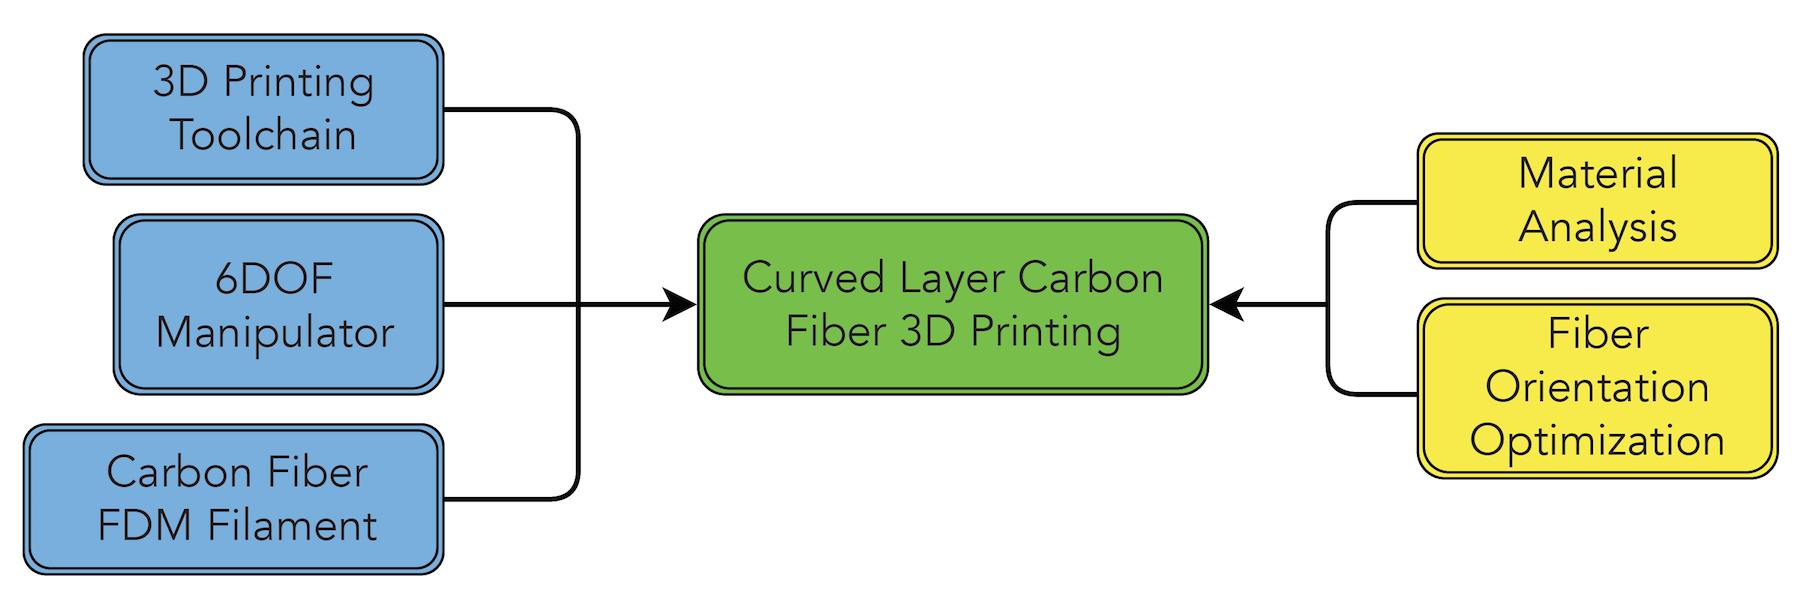
\includegraphics[width=0.75\textwidth]{./figures/flowchart}
%\caption{A flow chart of subsystems.}
%\label{fig:flowchart}
%\end{figure}

